\chapter{分子模拟——锂离子迁移过程中弹性常数计算及断裂行为模拟}
\section{研究背景}
锂离子电池的电极材料在锂离子的扩散过程,即电池的充放电循环中,其活性颗粒会有相当大的体积变化,以常见的负极材料石墨为例,其体积在锂离子的嵌入过程中会增加大约10\% \cite{Dahn1991Phase},而在锂离子的容纳量上超出石墨十倍的硅则在嵌入锂过程中会有高达300\% 的体积增长\cite{Beaulieu2003The}。
\begin{figure}
\centering   
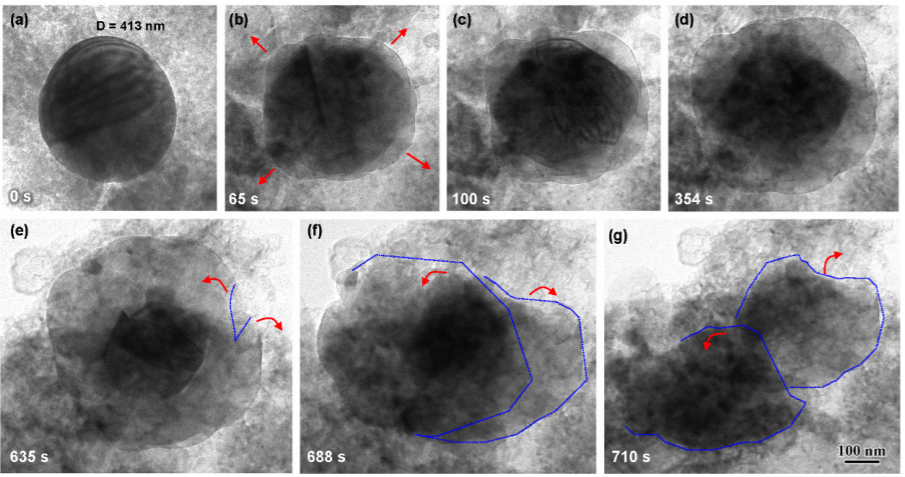
\includegraphics[width=0.8\textwidth]{Si.png}
\caption{硅颗粒在充放电过程中的开裂} 
\label{fig:Si}
\end{figure}
就微观层面上而言,锂离子电池的活性颗粒内部的力学强度在维持锂离子电池电极的力学完整性上有着重要的作用\cite{Lee2014Molecular}。由此可见,由于锂离子扩散(Li diffusion-induced stress, DIS)引起的应力是造成体积变化乃至电极断裂的重要因素。同时,由于应力产生和锂离子扩散过程的相互作用,使得这一问题涉及了力学、电化学乃至热力学多个方面物理因素的耦合。\\
\indent 近些年来,很多研究者希望通过调控DIS来增强锂离子电池的力学强度和耐久性\cite{Christensen2005A,Christensen2006Stress,Zhang2007Numerical,Verbrugge2009Stress,Cheng2008The,Zhang2008Intercalation}。如,Wolfenstine等人建立了基于杨氏模量、断裂强度乃至体积变化的对于颗粒尺寸影响容量消退的模型\cite{Woodford2010},Zhao等人则基于断裂力学和扩散动力学发展了判断钴酸锂颗粒断裂失效的准则\cite{Zhao2010Fracture}。 但是,这些研究的模型,多数只考虑体积变化造成的应力,从而不能真实反映实际复杂的电极材料的断裂失效行为。另外,这些模型都是基于固体扩散理论和连续介质力学的方程,需要一系列的诸如弹性常数(如弹性张量的分量,体材料的剪切和杨氏模量),表面能,扩散系数和体积膨胀率。 其中,模型中对于杨氏模量等力学参数的选取并未考虑其随着锂离子扩散的变化而给定为常值,这其实是因为处理不同SOC的电极材料进行力学特性的测试十分困难(由于锂离子和氧气的高度反应活性和制备大晶体的困难),从而应用数值模拟的手段得到这些参数和参数的动态变化就显得十分重要。\\
\indent如图\ref{fig:LiBattery}所示,在充放电过程中$LiFePO_4$电池会发生电极反应:
\begin{equation}
\label{eq:anode}
Anode : \quad Li_xC_6 -x e^{-} \to x Li^{+} +C_6
\end{equation}
\begin{equation}
\label{eq:cathode}
Cathode : \quad Li_{1-x}FePO_4 +x e^{-} + x Li^{+} \to LiFePO_4
\end{equation}
\indent 在充电时,外电压驱动锂离子从$LiFePO_4$晶体中脱出经过电解液到达石墨层,放电时则相反。显然,周期性的脱嵌和嵌入使得电极的正极和负极材料都会经历周期性的体积变化和诱导应力的产生,从而有可能造成电极材料的断裂失效进一步引起电池容量减小,这也是本章模拟需要揭示和研究的核心问题。

\begin{figure}
\centering   
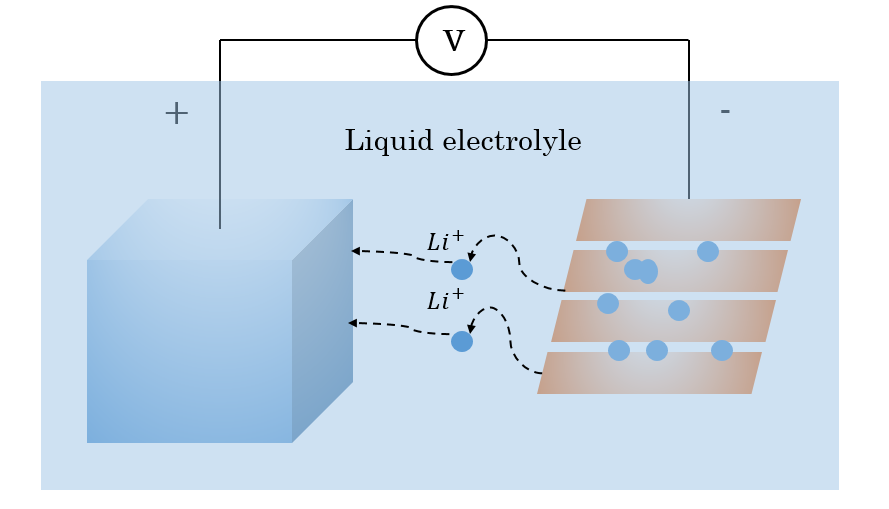
\includegraphics[width=0.8\textwidth]{LiBattery.png}
\caption{锂离子电池电化学通路示意图} 
\label{fig:LiBattery}
\end{figure}
\section{锂离子在磷酸亚铁锂晶体中的迁移过程及其弹性常数:密度泛函矩阵方法}
\subsection{简介:磷酸铁锂材料}
磷酸铁锂作为锂离子电池的电极材料其理论的容量为170mAh/g,其嵌锂电位为3.5V, 并有着很良好的热稳定性。 另外,磷酸铁锂由于其低廉的价格和相对的低污染成为了很多商用锂离子电池电极材料的选择。室温下,磷酸铁锂通过在磷酸铁和磷酸铁锂间的相变转换来进行充放电循环,其反应方程见方程\ref{eq:anode}和方程\ref{eq:cathode}。\\
\indent 磷酸铁锂属于正交晶系,其晶格常数为a = 10.3375 $\dot{A}$, b=6.0112$\dot{A}$, c= 4.6950 $\dot{A}$ 。 如图(\ref{fig:LiFe})所示,其内部的六方密排结构内部为被六个氧原子所围绕的亚铁离子,其又被磷酸基团所形成的四面体所分隔。
\begin{figure}
\centering   
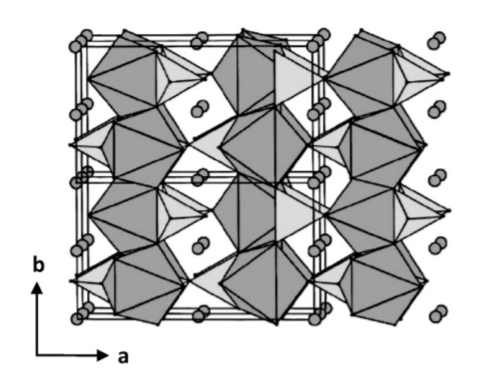
\includegraphics[width=0.6\textwidth]{LiFe.png}
\caption{$LiFePO_4$晶体结构,其中铁原子和磷原子分别占据八面体和四面体位置,锂离子嵌入其中的空隙\cite{Zhang2011Structure}} 
\label{fig:LiFe}
\end{figure}
\subsection{锂离子在两个晶体方向的输运模拟和计算}
本文的结构分析和离子扩散的计算模拟的密度泛函方法\cite{Kohn1965Self}(DFT)采用第一性计算软件包Vienna ab initio simulation package(VASP)的plane wave basis set\cite{Kresse1996Efficiency,Kresse1994Ab,Kresse1996Efficient}模拟,调用VNL进行后处理\cite{Schneider2017ATK,Stradi2017Method}和结果分析。在密度泛函计算中,利用Kohn-Sham方法将多体问题转化为一个假设虚拟粒子(如电子)在无相互作用的有效势场中运动,而粒子密度在空间中和真实系统相同的半经典近似方法\cite{Kohn1965Self}。在本文的求解中采用局域密度近似\cite{Vanderbilt1990Soft}(LDA)的求解方法进行求解。\\
\indent 首先本文进行锂离子在磷酸铁锂晶体中的扩散模拟,从而得到不同SOC的晶体结构为下一步的弹性常数的模拟和计算打好基础。
\begin{enumerate}
	\item 首先对于构建的$LiFePO_4$晶体结构进行弛豫优化:
	\begin{itemize}
		\item 采用SGGA-PBE 交换关联函数
		\item k-point取为$7 \times 5 \times 3$
		\item 应用FHI赝势和DZP基组模拟
	\end{itemize}
	具体的优化参数设定为 最大容许力为0.02 $eV/\dot{A}$,最大应力0.1$ GPa$。体系在八核CPU上耗费30分钟完成结构弛豫。
	\begin{figure}
	\centering   
	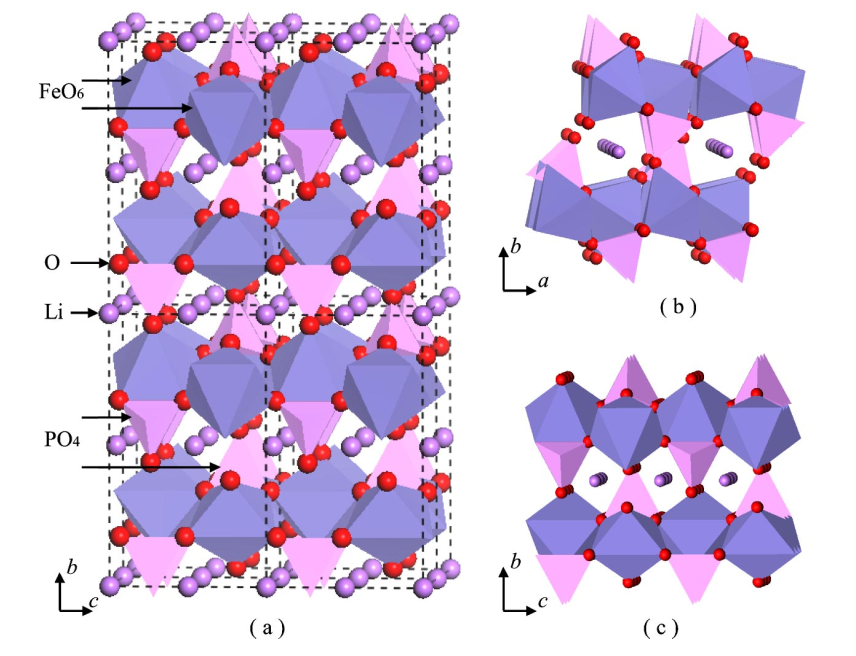
\includegraphics[width=0.6\textwidth]{diffusion.png}
	\caption{$LiFePO_4$晶体a,b,c三方向结构\cite{Ouyang2004First}} 
	\label{fig:diffusion}
	\end{figure}
	\item 文献指出,扩散势垒和锂离子的聚集形态有关\cite{Ouyang2004First},所以为了模拟锂离子的扩散过程,可以在晶格中去除四个锂离子的其中一个得到$Li_{1-x}FePO_4$的结构。如图(\ref{fig:diffusion})所示,本文将对锂离子在B,C两个方向的扩散进行研究,为此需要创建锂离子在两个方向扩散的前后的晶体构型。\\
	\begin{figure}
	\centering   
	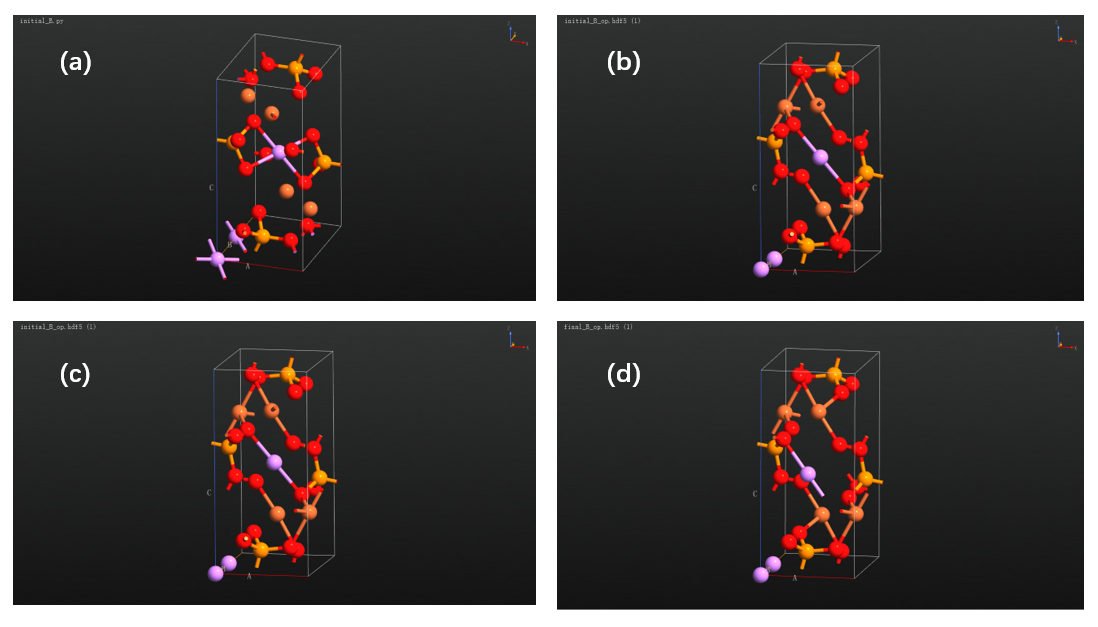
\includegraphics[width=\textwidth]{trace.png}
	\caption{$LiFePO_4$晶体B方向锂离子扩散前后结构:(a)扩散前(未优化)\quad(b)扩散前(优化后)\quad(c)扩散后(未优化)\quad (d)扩散后(优化后)}
	\label{fig:trace}
	\end{figure}
	以B方向的构型构造为例:
	\begin{itemize}
		\item 借助引入重金属原子如Au原子得到删去某个锂原子的晶格构型,由此得到B方向的扩散的起始和终了构型的初步结构(\ref{fig:trace}(a)(c))。
		\item 对得到的两个构型的结构进行弛豫优化,需要注意的是,此处不需要对晶格常数进行优化,最后得到优化后的扩散起始和终了构型的结构(\ref{fig:trace}(b)(d))。
		\item 再通过微动弹性带方法(Nudged Elastic Band,NEB)从之前的初始构型得到扩散过程的路径和相关晶格构型\cite{Smidstrup2014Improved,Zhou2004Misfit,Kellogg1990Surface}。实际上,该方法通常需要一个基于初始和终了构型的对于可能路径的猜测而这往往是十分困难的,而实际上可以依靠自适应动力学蒙特卡洛(Adaptive Kinetic Monte Carlo,AKMC)的方法获得额外的信息从而帮助计算\cite{Xu2008Adaptive,Henkelman1999A}。对于微动弹性方法的介绍和如何应用来解决扩散路径问题的内容见附录B。
	\end{itemize}
	\item 获得构型和扩散路径后,可以利用DFT方法计算得到其扩散过程中的能量变化,如图所示\ref{fig:energy}(a)(b):
	\begin{figure}
	\centering   
	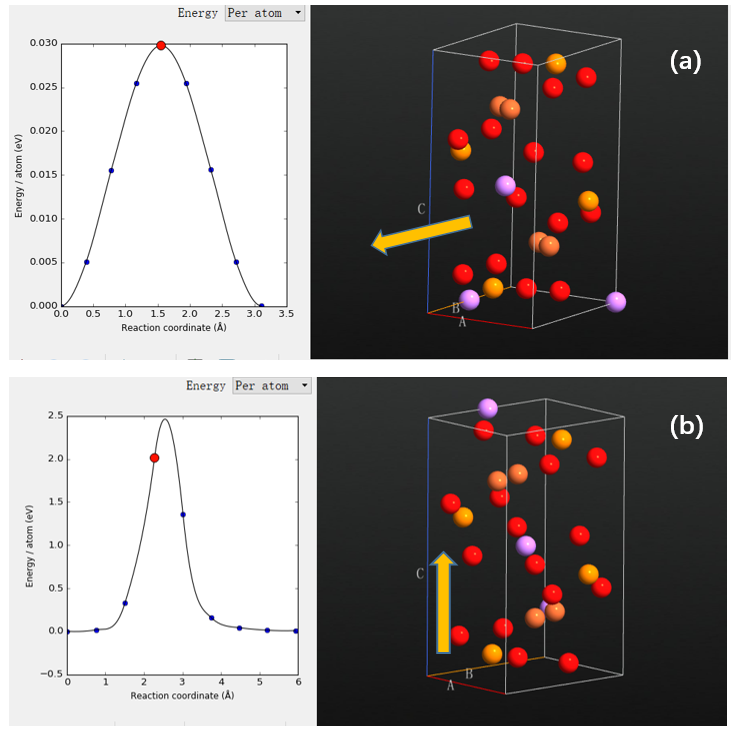
\includegraphics[width=0.8\textwidth]{energy.png}
	\caption{$LiFePO_4$晶体B方向和C方向锂离子扩散过程} 
	\label{fig:energy}
	\end{figure}
	可以看出,由于较小的势垒,锂离子在B方向的扩散要比在C方向扩散要容易很多。
	\item 基于前面对于扩散过程能量势垒的研究,从微观上而言,锂离子的扩散主要依赖势垒高低,从宏观上而言,这一参数可以用电化学反应的速率来很好的描述。基于此,本文采用谐波过渡态理论(Harmonic Transition State Theory,HTST)来计算两个扩散方向的反应速率\cite{Vineyard1957Frequency,Eyring1935The,Voter1984Transition}(较为详细的计算过程见附录B)。两个方向的结果见图\ref{fig:reaction},可以看出B方向的反应速率远远高于C方向,和微观的势垒分析的结果一致。
	\begin{figure}
	\centering   
	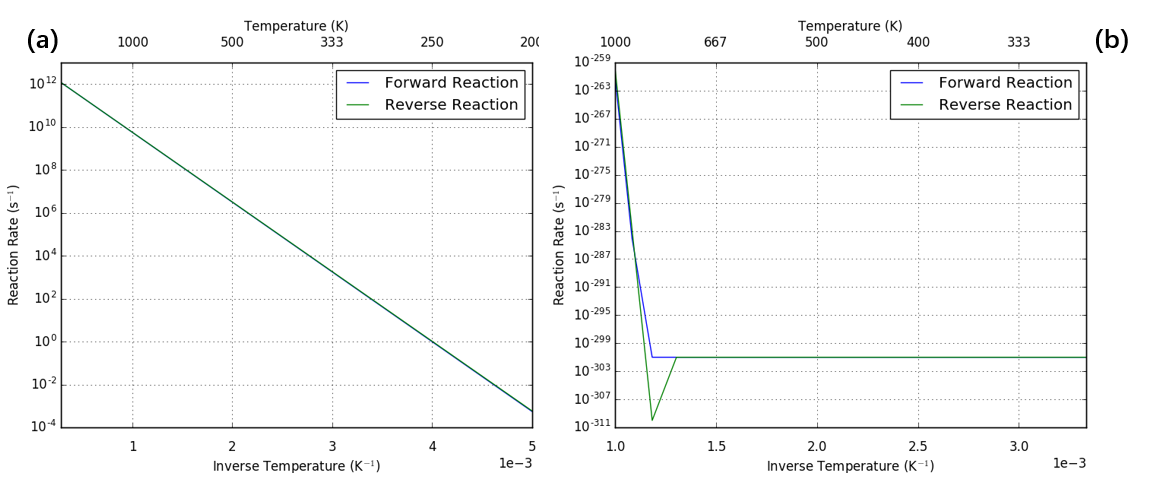
\includegraphics[width=\textwidth]{reaction.png}
	\caption{$LiFePO_4$晶体B方向和C方向反应速率图:(a)B方向 (c)C方向} 
	\label{fig:reaction}
	\end{figure}
\end{enumerate}
\indent以上基于第一性原理对于锂离子在$LiFePO_4$晶体B和C两个方向的扩散输运的在300k下的势垒和反应速率可以总结如表\ref{tab:HTST}:
\begin{table}
	\centering
	\caption{势垒和反应速率}
    \label{tab:HTST}
    \begin{tabular}{ | c | c | c | }
    \hline
    \hline
    Direction & Barrier(eV) & $k_{HTST}$\\ \hline \hline
    B & 0.03 & $2.5 \times 10^6$\\
    C & 2.5 & $10^{-300}$ \\
    \hline
    \hline
    \end{tabular}
\end{table}
\subsection{弹性常数的计算及各向异性分析}
\subsubsection{线弹性关系}
对于晶体而言,其在一定的范围内都很好的满足线弹性的关系,则应力和应变都是二阶张量,其在空间中均有九个分量,可以用Voigt notation表示为下列形式:
\begin{equation}
\label{eq:stress}
\mathbf{\sigma} =\left( \sigma_{xx}, \sigma_{yy}, \sigma_{zz}, \sigma_{yz}, \sigma_{xz}, \sigma_{xy} \right)
\end{equation}
\begin{equation}
\label{eq:strain}
\mathbf{\epsilon} =\left( \epsilon_{xx}, \epsilon_{yy}, \epsilon_{zz}, 2\epsilon_{yz}, 2\epsilon_{xz}, 2\epsilon_{xy} \right)
\end{equation}
由张量理论,应变张量和应力张量之间由弹性矩阵相关联,弹性矩阵为一个四阶张量,表现为一个$6 \times 6$的矩阵,其中的元素称为弹性常数。
\begin{equation}
\label{eq:rule}
\mathbf{\sigma} = \mathbf{C} \cdot \mathbf{\epsilon} 
\end{equation}
由于晶体均有对称性,所以很多时候,弹性矩阵中的独立参数的数目可以被缩减。比如,对于立方晶系而言,只有$C_{11}$,$C_{12}$,$C_{44}$是独立的,此时方程\ref{eq:rule}可以简化为:
\begin{equation}
\begin{pmatrix}
\sigma_1\\
\sigma_2\\
\sigma_3\\
\sigma_4\\
\sigma_5\\
\sigma_6\\
\end{pmatrix}
=
\begin{pmatrix}
C_{11} & C_{12} & C_{12} & 0 & 0 & 0\\
C_{12} & C_{11} & C_{12} & 0 & 0 & 0\\
C_{12} & C_{12} & C_{11} & 0 & 0 & 0\\
0&0&0& C_{44} & 0 & 0\\
0&0&0& 0 &C_{44} & 0 \\
0&0&0& 0 & 0& C_{44} \\
\end{pmatrix}
\begin{pmatrix}
\epsilon_1\\
\epsilon_2\\
\epsilon_3\\
\epsilon_4\\
\epsilon_5\\
\epsilon_6\\
\end{pmatrix}
\end{equation}
\subsubsection{模拟过程}
\indent 在模拟中,为了求解得到弹性常数,首先在选定的方向给定晶格微小的形变,如$\mathbf{\eta}$,然后求解产生的应力向量。然后再对每一个应变向量下的应力分量$\sigma_i(\eta)$做拟合,这样就可以再通过求解一系列的考虑了具体晶格结构的线性方程组的最小二乘解得到所相互独立的弹性常数。在计算中,模拟程序实际采用的是文献所推荐的计算弹性常数的ULICS方法\cite{Yu2010Calculations},即每一个参考点,所给定的初始变形为$(-\eta,0,\eta)$。\\
\indent 实际上,在单轴加载的情况下$(\epsilon_{22}=\epsilon_{33}=0,\epsilon_{11} \not \eq 0)$,x方向的应力就可以表示为:
\begin{equation}
\sigma_{11} = C_{11}\epsilon_{11}
\end{equation}
进而可以计算体弹模量 $K$ 为:
\begin{equation}
K = \frac{1}{3} \left(\frac{\sigma_{11}+\sigma_{22}+\sigma_{33}}{\epsilon_{11}+\epsilon_{22}+\epsilon_{33}} \right)
\end{equation}
可以看出,可以建立弹性常数$C_{11}$和体弹模量$K$和应力应变的关系,从而进一步可以得到$C_{11}$和$K$和宏观材料力学参数杨氏模量和泊松比的关系(对于各向同性材料而言):
\begin{equation}
\label{eq:C11}
C_{11} =\frac{(1- \nu)E}{(1+\nu)(1-2\nu)}
\end{equation}
\begin{equation}
\label{eq:K}
K = \frac{E}{3(1-2\nu)}
\end{equation}
从方程\ref{eq:C11}和\ref{eq:K}可以得出,等效杨氏模量可以由下式求得:
\begin{equation}
E = \frac{9K(C_{11}-K)}{3K + C_{11}}
\end{equation}
\indent 弹性常数的第一性原理模拟中涉及具体模拟参数的设置,讨论如下:
\begin{itemize}
	\item $\mathbf{\eta_{max}}$ \\
	表征了对晶格所施加的最大变形,显然,只要限制在线弹性的区域内,相对较大的变形会得到比较好的应力变化从而得到比较准确的弹性常数。 根据之前的对于晶体的计算经验,通常而言默认取值为$\eta_{max} = 0.002$。
	\item $\mathbf{\eta_{\eta}}$\\
	该参数为施加变形场时的差分间隔,即可以通过$\eta_{\eta}$和$-\eta_{max},\eta_{max}$求得所需要具体计算的每一个形变量。 当然,采用相对密集的取点(即相对比较小的$\eta_{\eta}$的取值)和高阶的插值函数可以增加精度。但是由于此处不需要模拟非线性(如塑性)行为,只需要取到$\eta_{\eta}=3$即可。
\end{itemize}
\subsubsection{计算结果和分析}
由于本文研究锂离子扩散过程对路径基于NEB方法进行了详细而比较准确的模拟,所以可以得到整个扩散过程的晶体构型,从而可以分别对每一个构型进行弹性常数的计算。需要指出的是,由于电极材料所面临的核心难题为锂离子在扩散过程中电极材料的断裂,所以对于扩散过程和力学特性进行耦合研究显得十分必要,特别是,基于本文的研究思路的方法,可以得到电极活性材料(此处为$LiFePO_4$)随着锂离子的扩散而产生的力学特性的动态变化,从而进行一下一部的耦合研究和分析建模。\\
\begin{figure}
	\centering   
	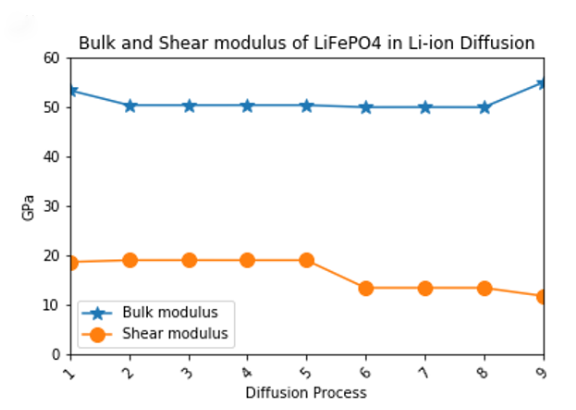
\includegraphics[width=\textwidth]{modulus.png}
	\caption{$LiFePO_4$晶体在锂离子扩散过程中其三个方向弹性模量和体弹模量和剪切模量的变化} 
	\label{fig:modulus}
\end{figure}
\indent 如图\ref{fig:modulus}所示,本文分析了在锂离子沿着B方向扩散过程中晶体的弹性参数的变化,可以看出在锂离子的扩散行为和晶体的力学特性的耦合特性。具体分析发现,其模量基本上都在扩散过程中有着下降的趋势,可能是由于扩散时成键较弱此时抵抗外界变形的能力相对减弱,从而其模量变小。定量的分析可以发现,在整个扩散过程中,三个方向的杨氏模量分别最小为之前的$77.65\%$,$91.18\%$和$95.32\%$,也就是说其模量会有最高$23\%$的减小。\\
\indent 另一方面,对弹性常数的计算分析可以知道,$LiFePO_4$晶体有着很强的力学各向异性。 而研究指出,作为锂离子电池的电极材料,随着锂离子在其中的扩散,由于其各向异性,会促使裂纹的形成和发展\cite{Tvergaard1988Microcracking,Rice1992Dislocation},从而使得电极活性材料失效乃至电池容量减退。对正交晶系的材料而言,其各向异性分为剪切产生和各向体弹模量非线性产生,
一般可以定义以下三个各向异性因子进行表征\cite{Ranganathan2008Universal,Ravindran1998Density}:
\begin{equation}
A_1 = 4c_{44}/(c_{11} + c_{33} -2c_{13})
\end{equation}
表征\{100\}平面的<010>和<011>方向
\begin{equation}
A_2 = 4c_{55}/(c_{22} + c_{33} -2c_{23})
\end{equation}
表征\{010\}平面的<001>和<101>方向
\begin{equation}
A_3 = 4c_{66}/(c_{11} + c_{22} -2c_{12})
\end{equation}
表征\{001\}平面的<010>和<110>方向\\
\indent 选取扩散过程中的四个代表结构进行三个各向异性因子的计算,其结果见表\ref{tab:A},同时也利用\cite{jerkwin}提供的各向异性晶体弹性常数可视化的方法绘制出以上四个结构的图像\ref{fig:mat}。

\begin{table}
	\centering
	\caption{各向异性系数}
    \label{tab:A}
    \begin{tabular}{ | c | c | c | c |}
    \hline
    \hline
    Sample & $A_1$ & $A_2$ & $A_3$\\ \hline \hline
    1 & -2.0899 & 0.5637 & 0.4491\\
    2 & -2.1834 & 1.0742 & 0.4423 \\
    3 & -2.7376 & 1.0575 & 0.3800\\
   	4 & -2.7480 & 0.9571 & 0.4618\\
    \hline
    \hline
    \end{tabular}
\end{table}

\begin{figure}
  \centering
  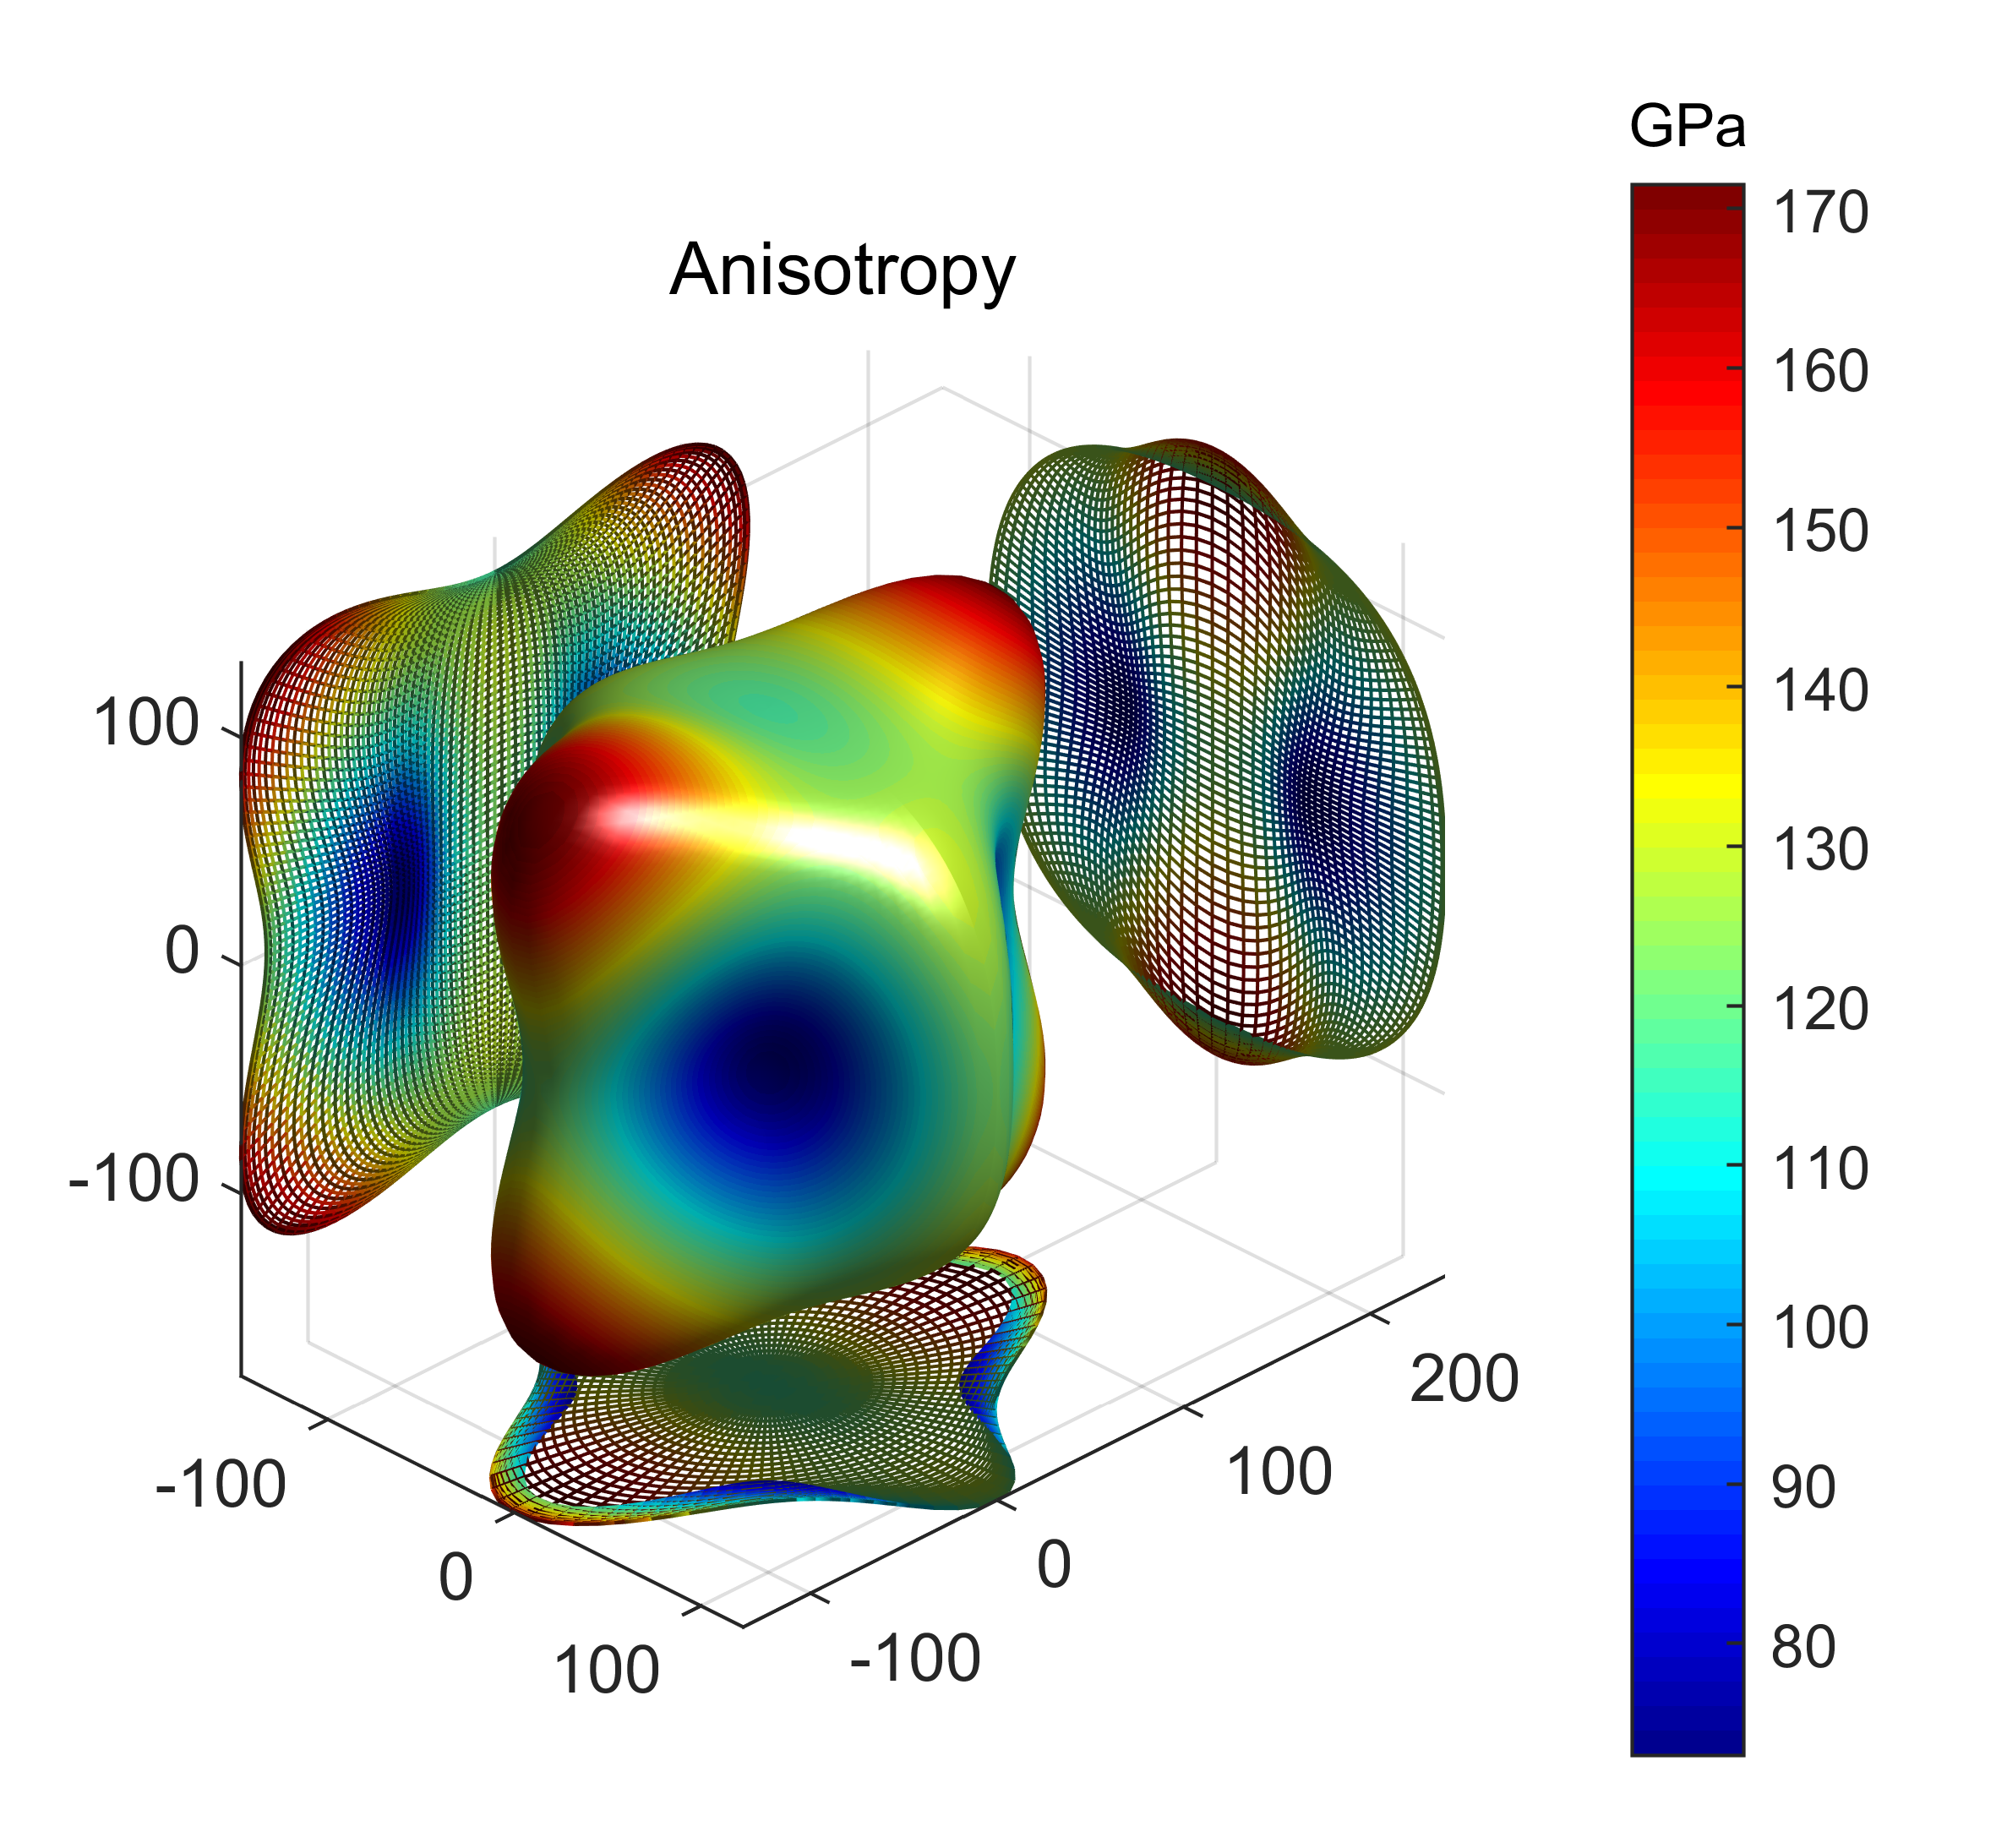
\includegraphics[width=.4\linewidth - 0.25mm]{1.png}\hfill
  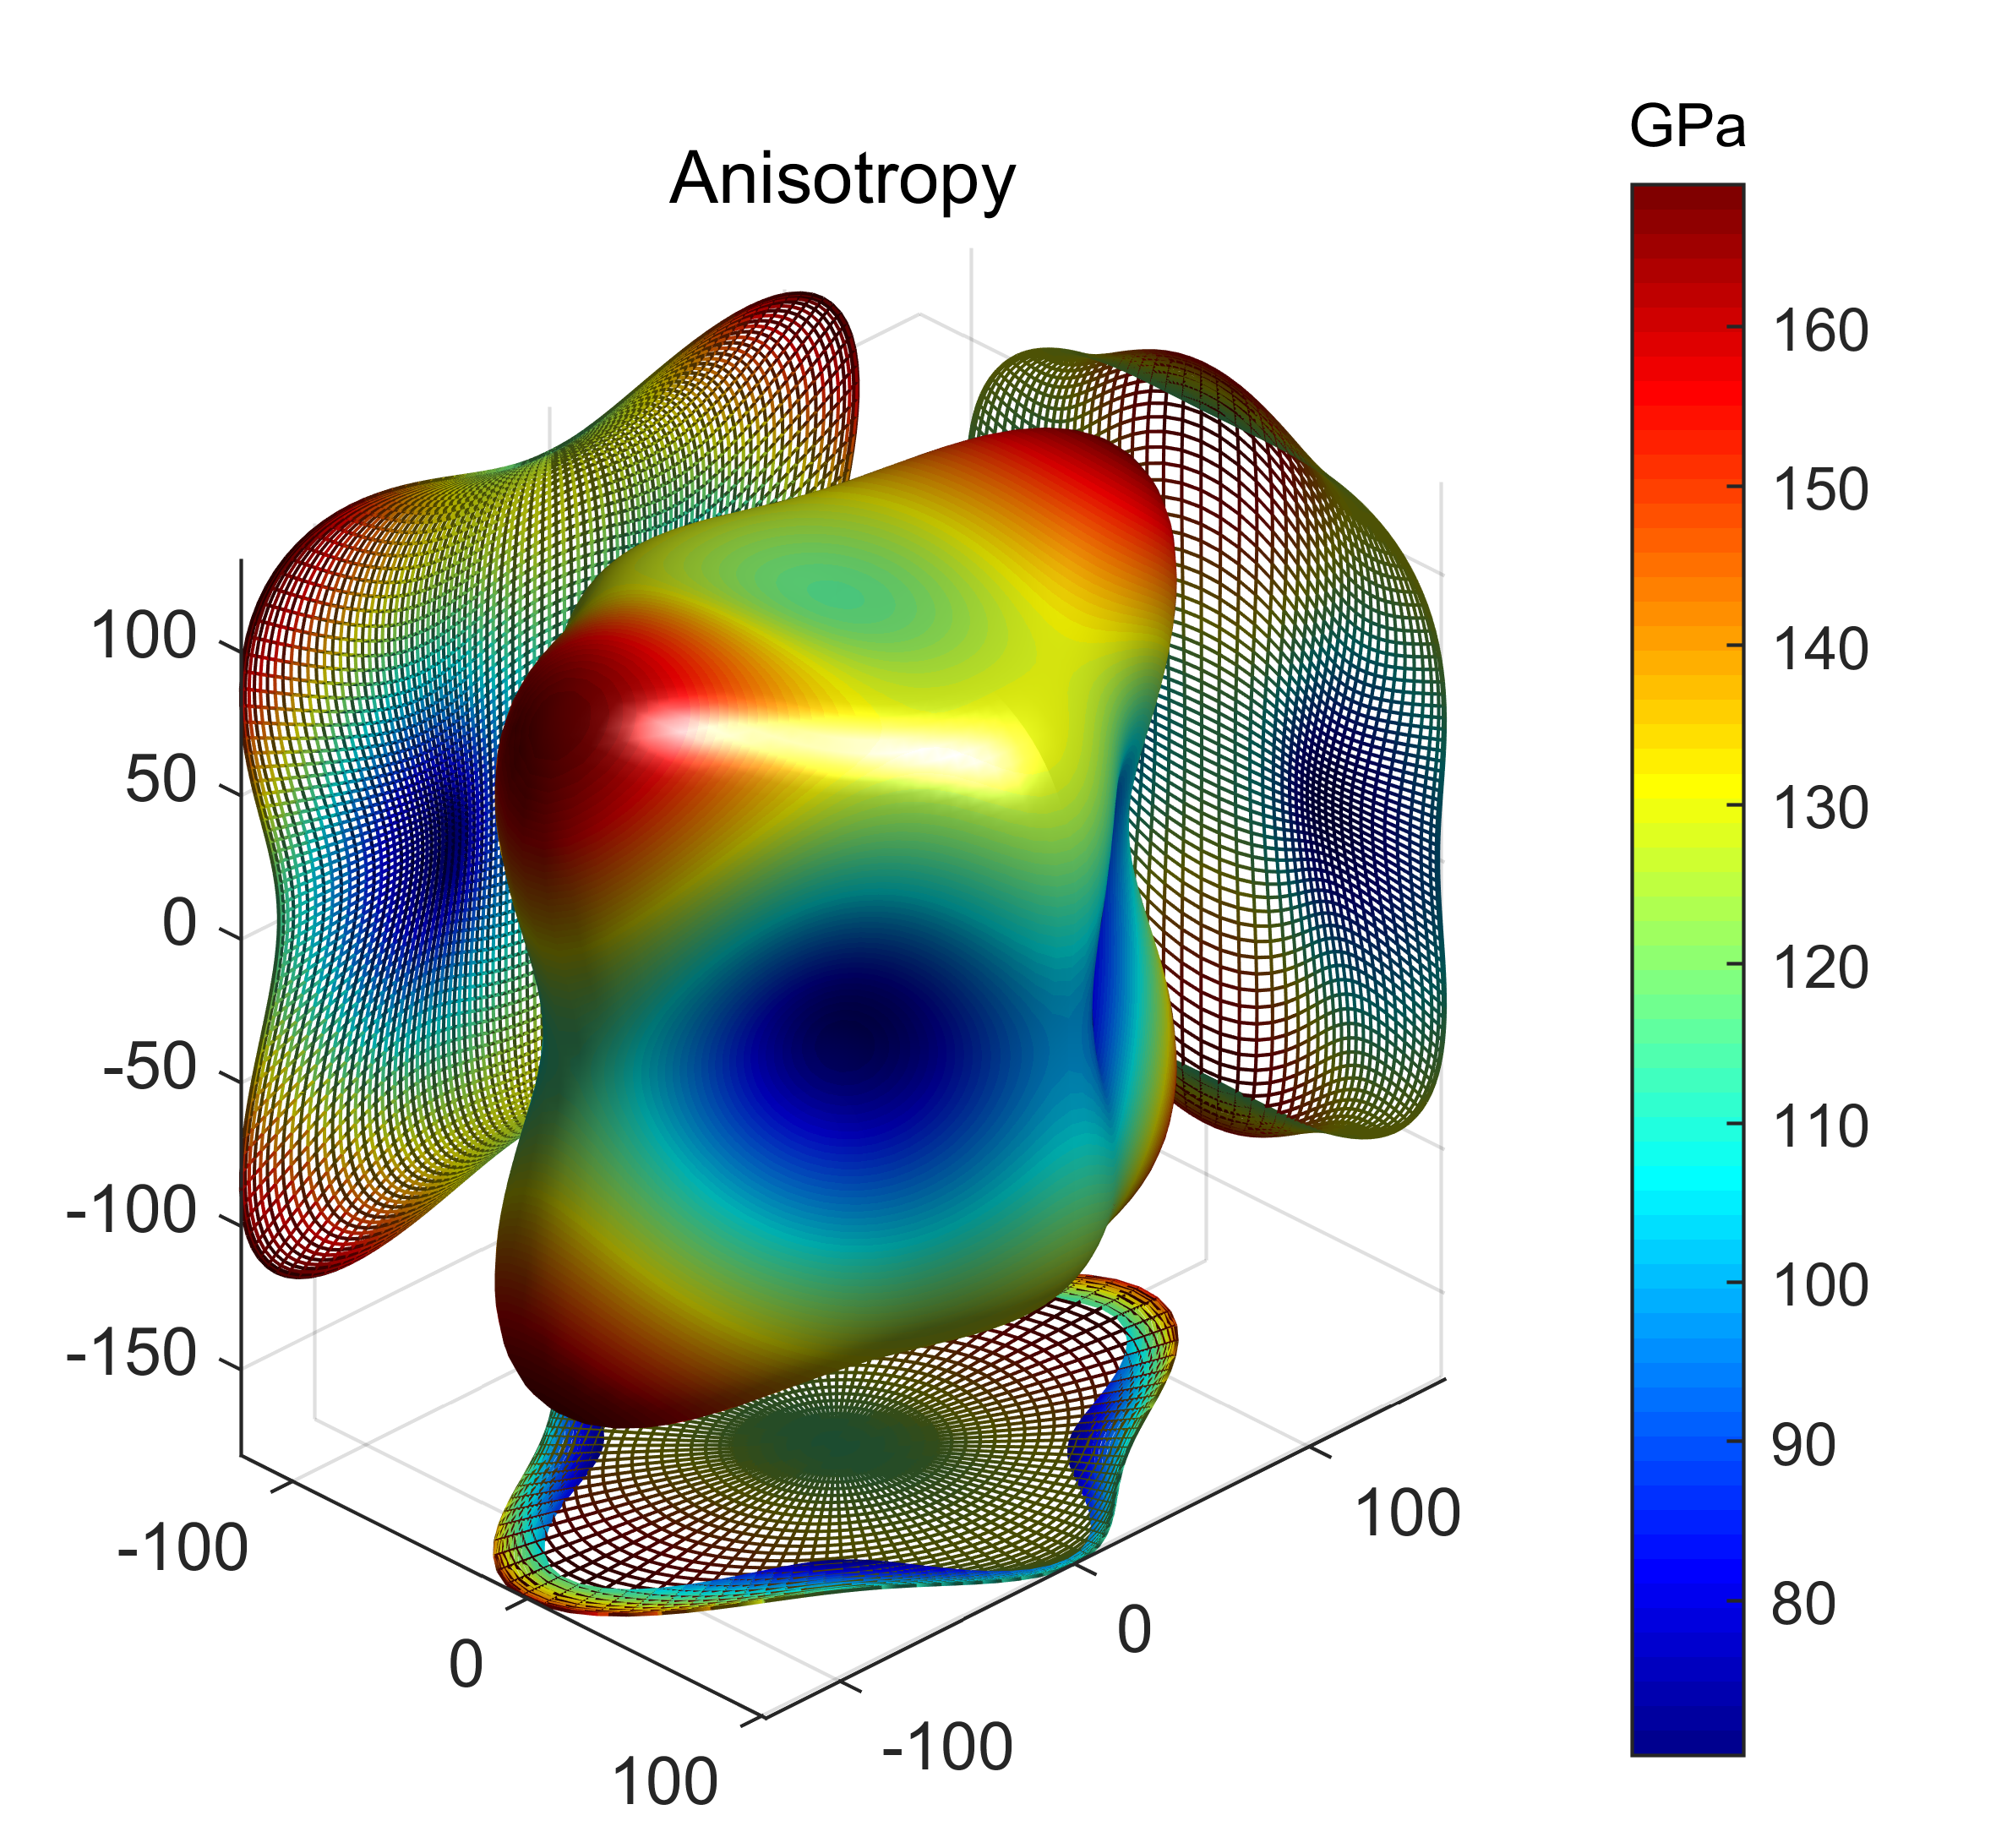
\includegraphics[width=.4\linewidth - 0.25mm]{2.png}\\[0.5mm]
  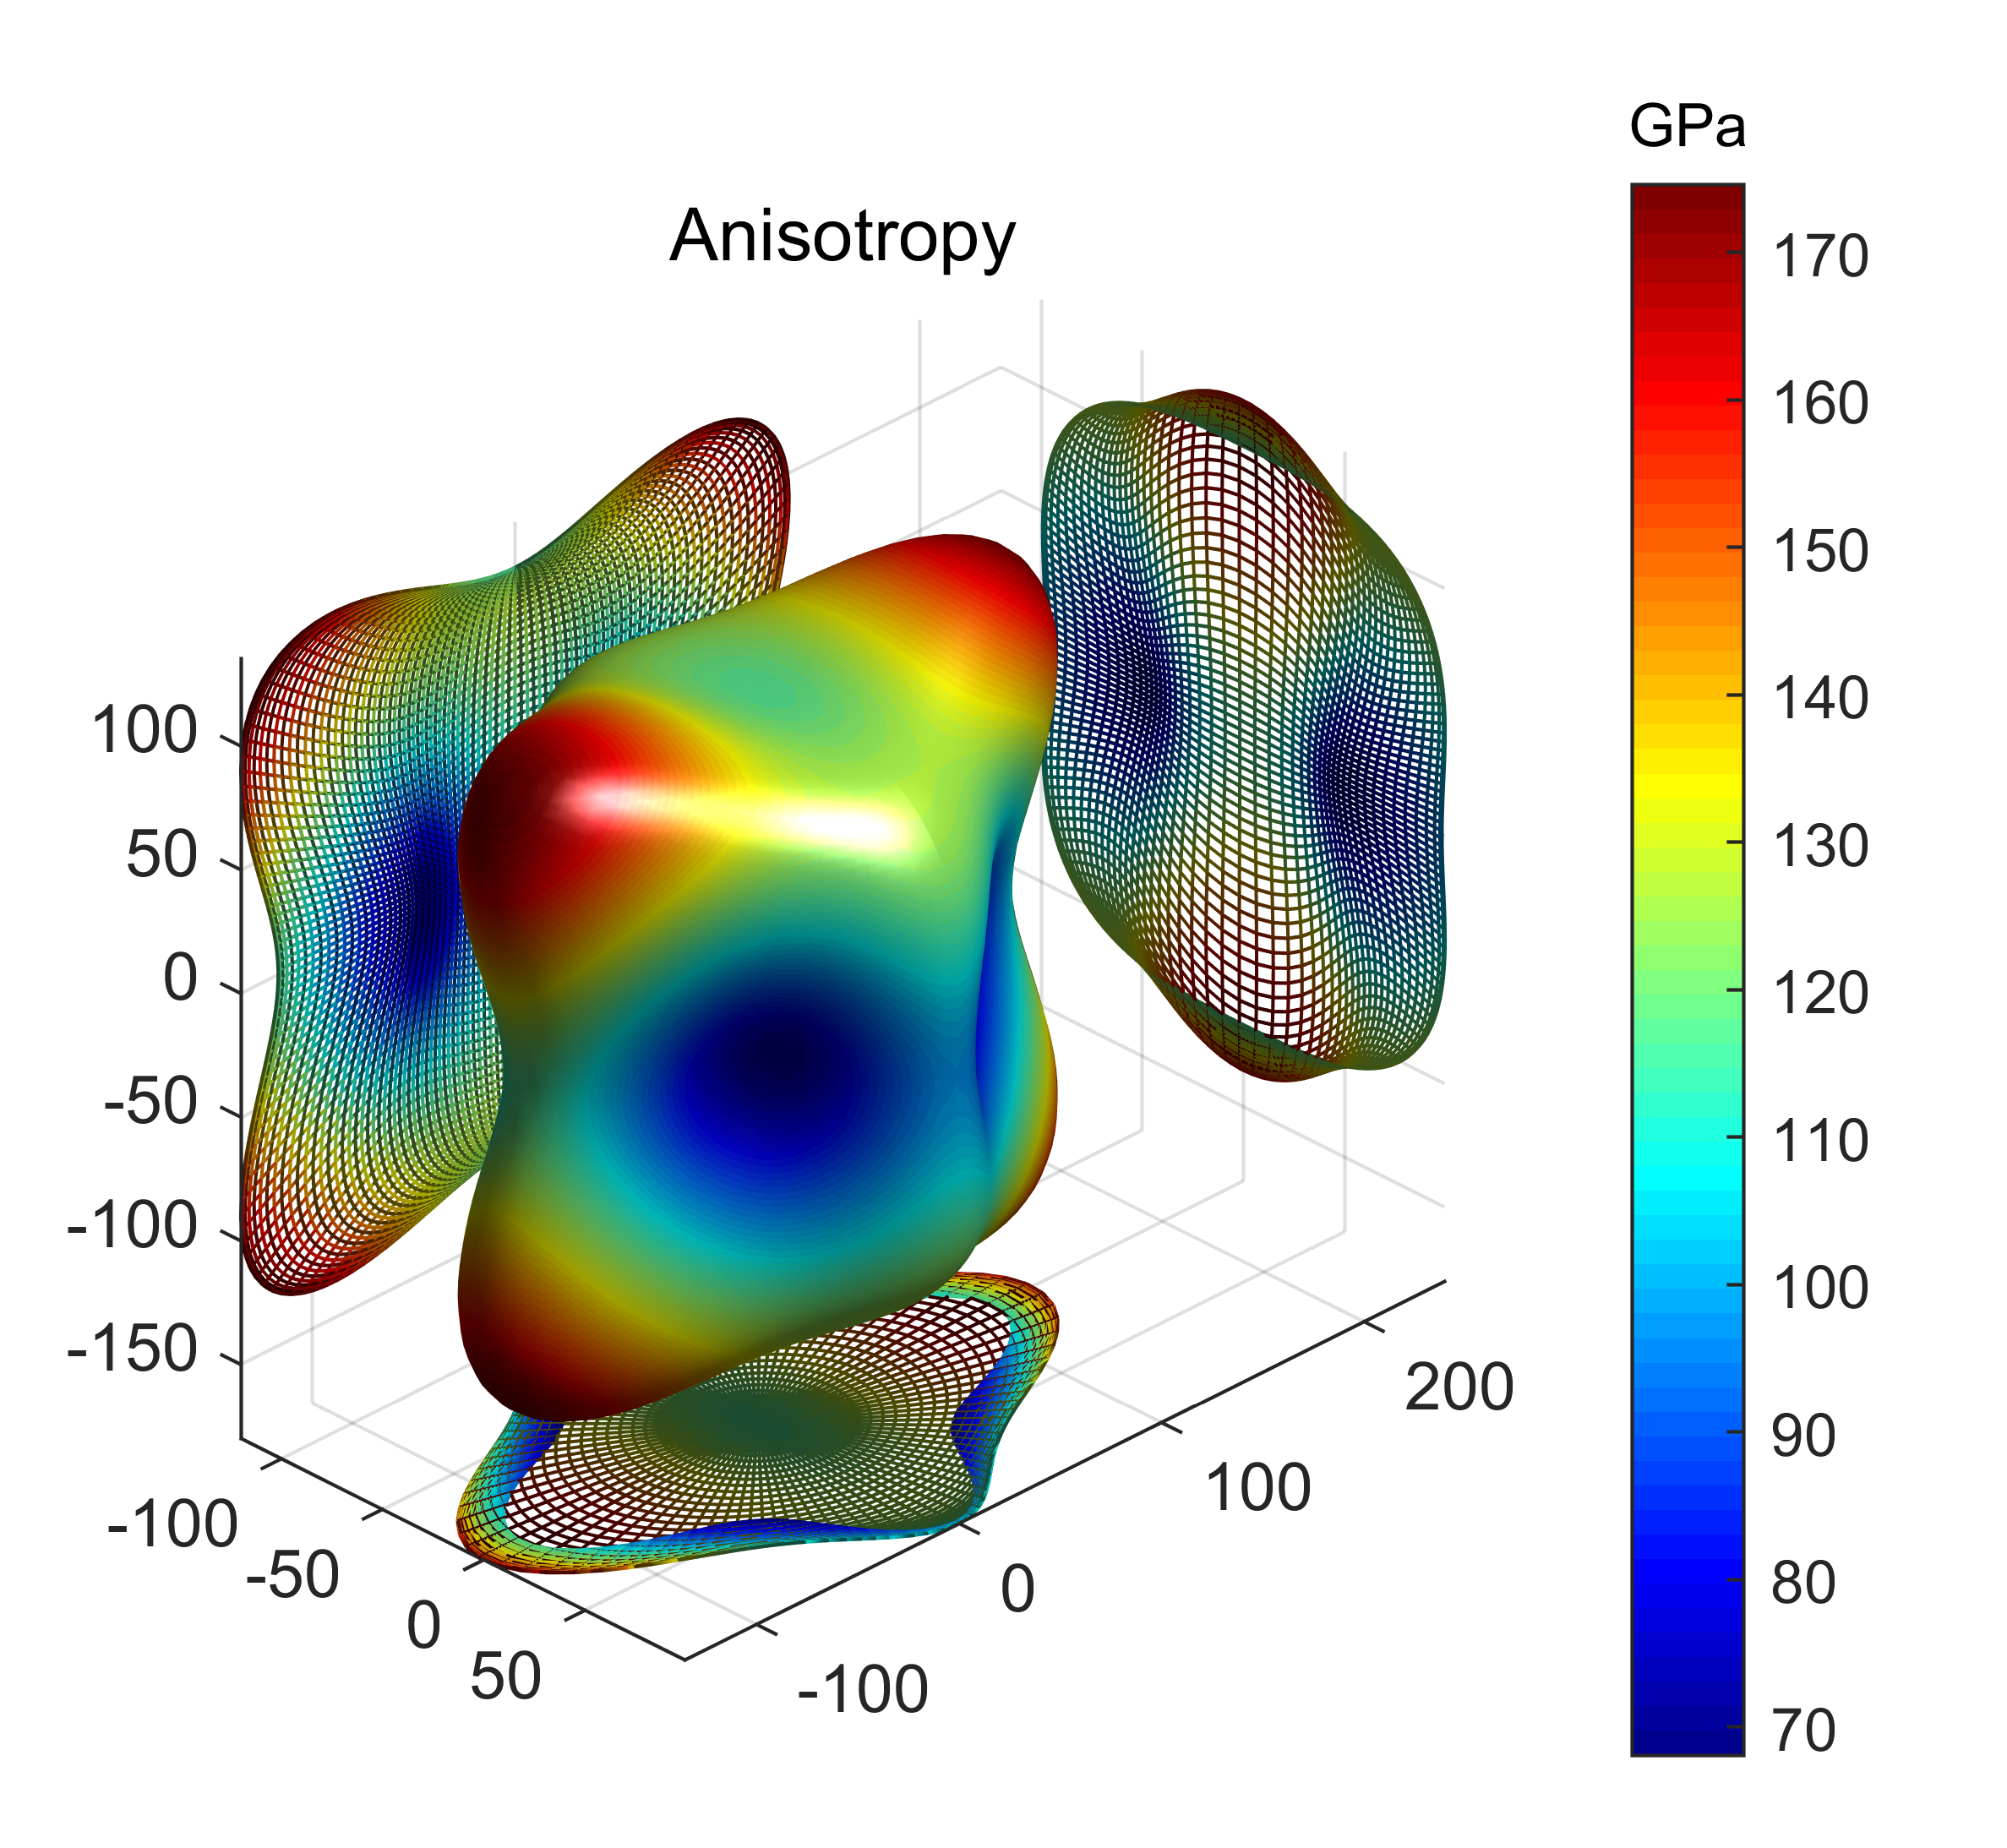
\includegraphics[width=.4\linewidth - 0.25mm]{3.png}\hfill
  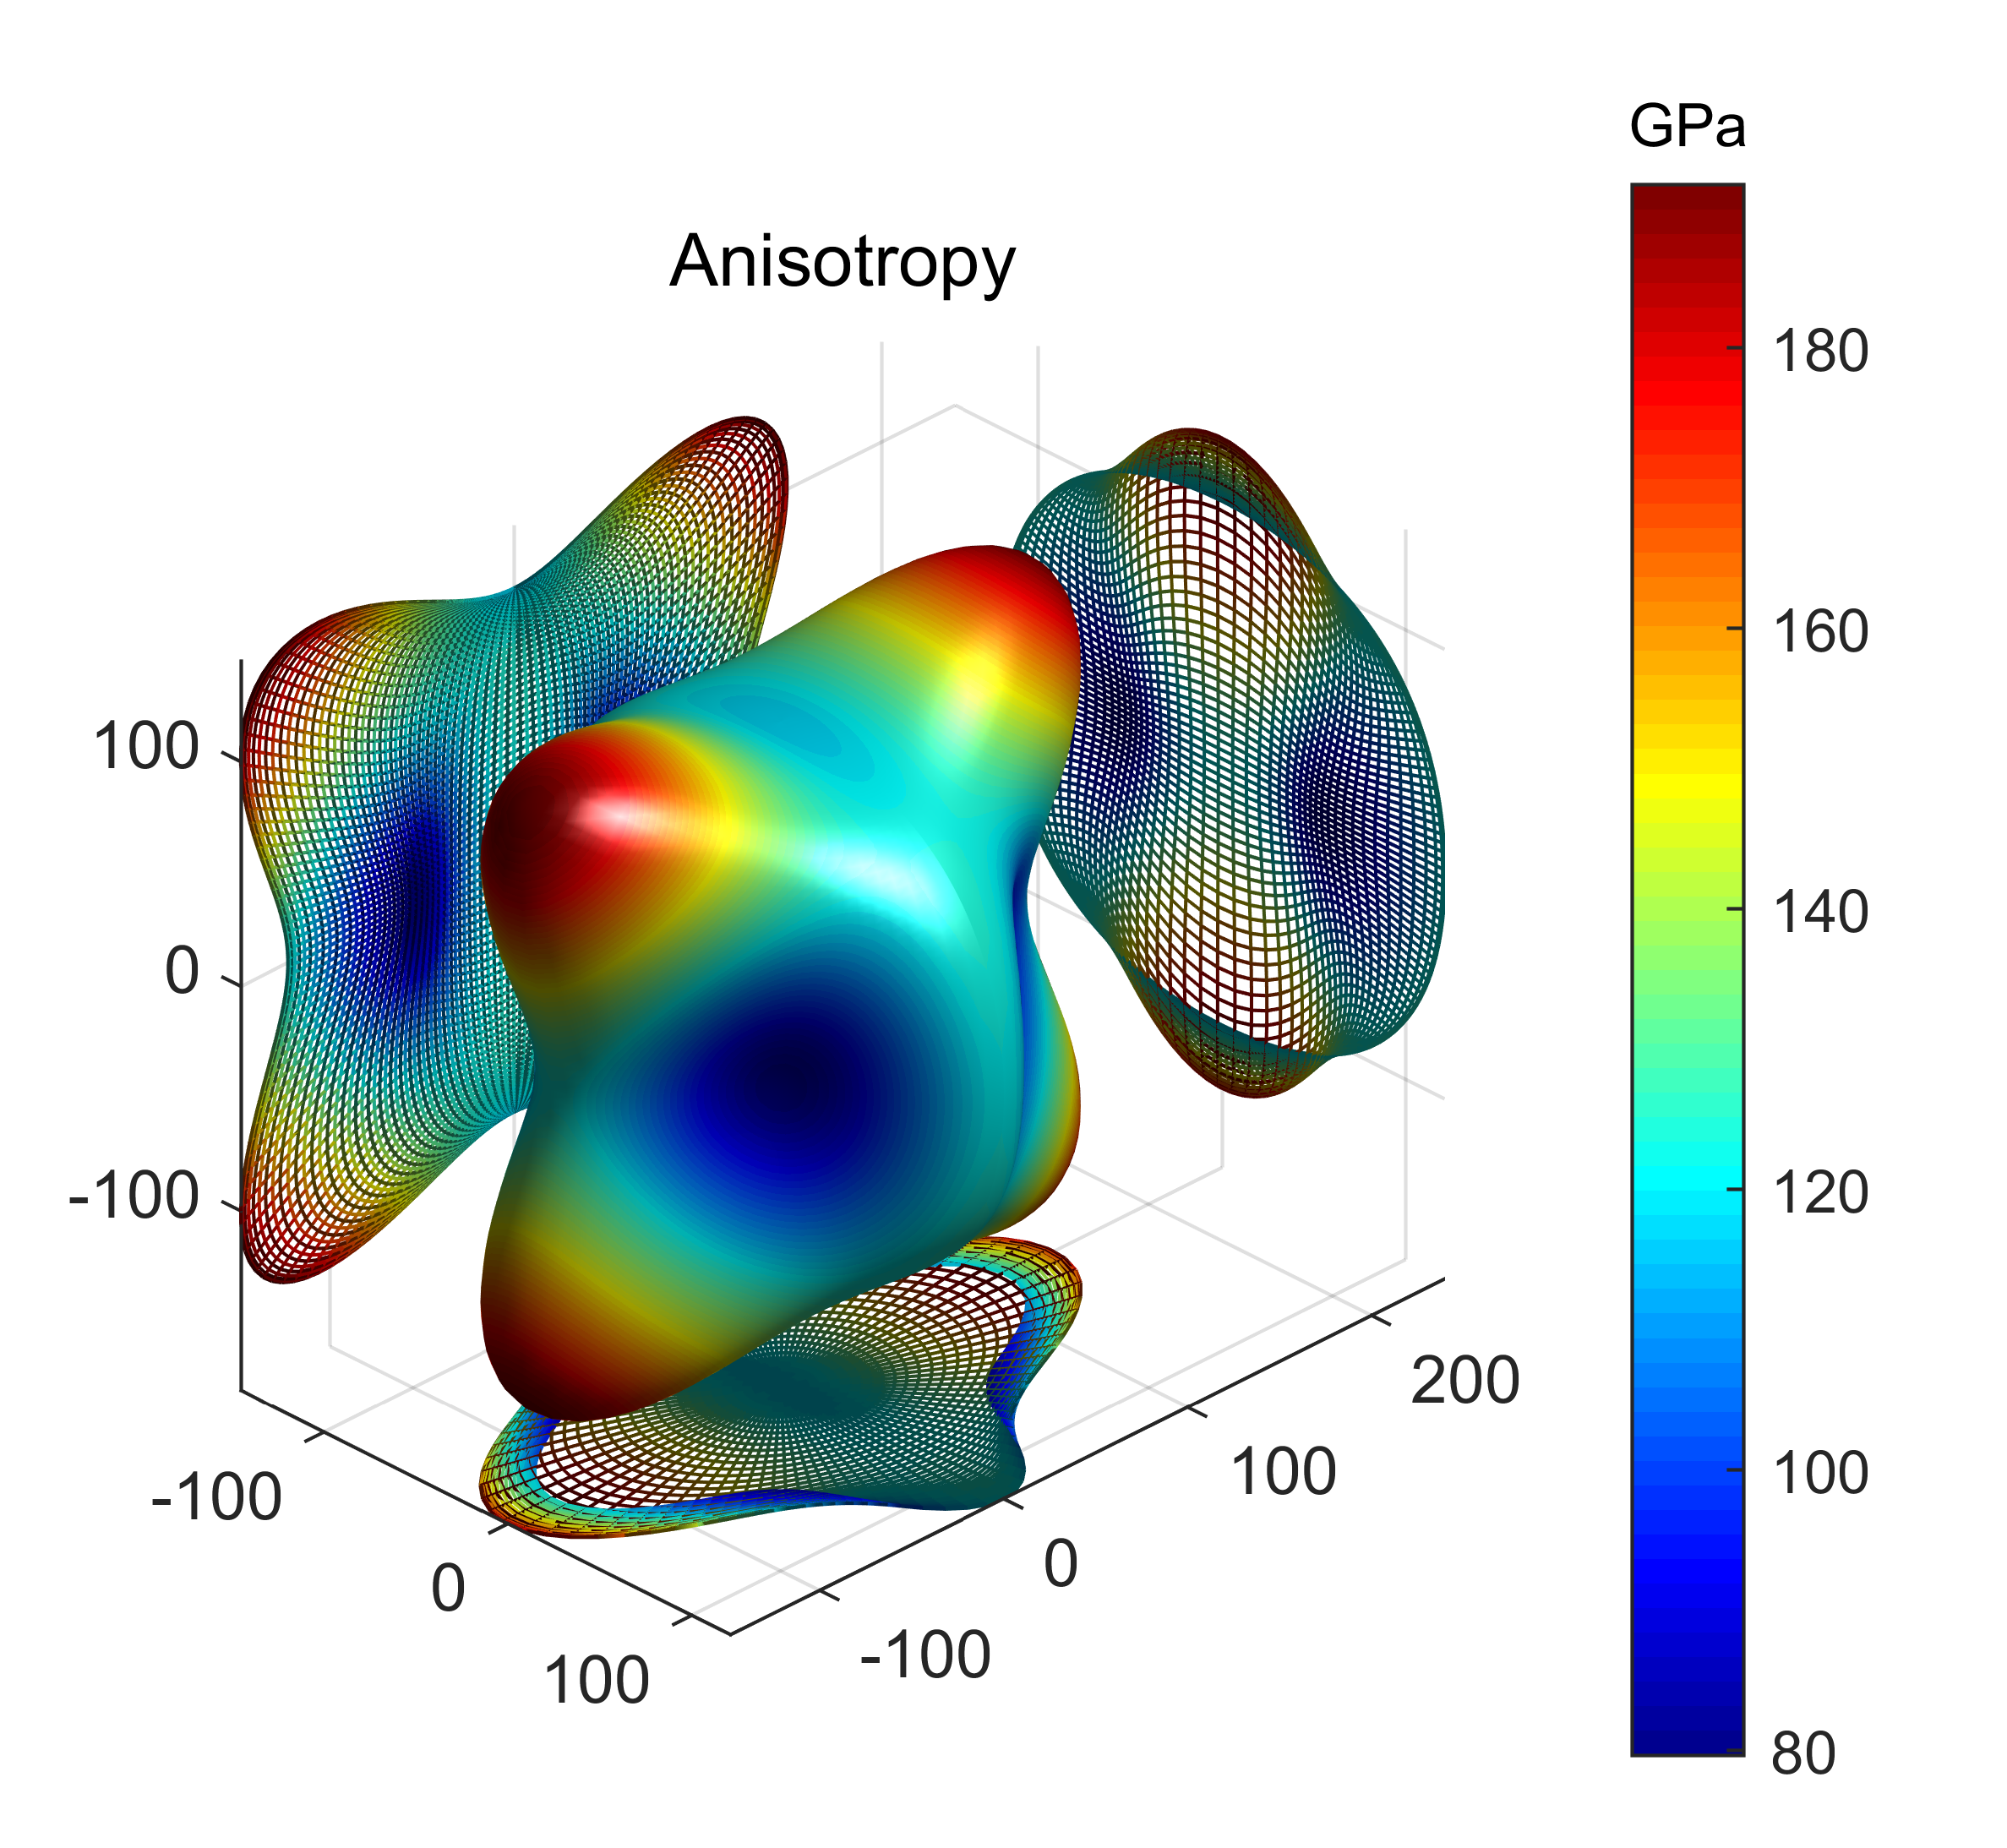
\includegraphics[width=.4\linewidth - 0.25mm]{4.png}
  \caption{$LiFePO_4$晶体在锂离子扩散过程中其三个方向弹性模量和体弹模量和剪切模量的变化} 
	\label{fig:mat}
\end{figure}






\section{不同SOC下的LiFePO4晶体力学响应的模拟研究:分子动力学模拟}
\subsection{模拟方法:分子动力学计算}
由于控制不同的SOC\cite{Qi2010Threefold}和制备磷酸铁锂大单晶十分困难,$LiFePO_4$的力学特性对于不同SOC的依赖特性少有实验研究。而分子动力学模拟则是求解这一问题的有效手段。\\
\indent 前文对锂离子扩散过程中的弹性特性进行研究,通过第一性原理计算的方法得到了锂离子扩散过程中的不同阶段晶格的弹性常数并以之为基础得到了弹性参数,总结出了电化学和力学所耦合的规律,而这里本文将对晶体结构的外力加载的力学响应行为进行模拟,主要得到其失效特性以及其塑性行为。而对这一问题,分子动力学由于其适应相对较大的体系研究,计算速度较快和计算效率较高的特点很适合这一问题的模拟和研究。需要指出的是,除了有着相对较快的计算速度和相对较大的模拟规模,在分子动力学模拟中,由于体系能量,应力等物理量都是分子坐标的光滑和连续函数,使得对于预先给定应变求解应力的算法有着很好的稳定性。\\
\indent  首先,本文对之前的扩散研究得到锂离子扩散前后的晶格构型进行弛豫。 需要指出的是,由于磷酸铁锂结构的复杂性,需要对每一种构型进行足够时间的弛豫。与基于量子力学的计算相比,由于预先定义的经验势能,所以计算的成本大为下降,可以在可以接受的时间和空间成本的花费下进行相对较大体系的模拟。\\
\subsubsection*{分子动力学}
分子模拟的势能项采用考虑了(1)长程作用的Coulomb势能 (2)短程作用的Morse函数 (3)附加项 $C/r^{12}$,呈现以下形式\cite{Alfonso2006A}:
\begin{equation}
\label{eq:MD}
U(r) = \frac{z_i z_j e^2}{r} +D_{ij} \left[\{1-e^{-a_{ij}(r-r_0)}\}^2 -1 \right] + \frac{C_{ij}}{r^{12}}
\end{equation}
\\
其中,第一项表征了静电相互作用,$Z_i$代表着原子的电荷,$e$为电荷常数,$r_{ij}$是原子$i$和原子$j$的原子间距;第二项表征了共价相互作用,$D_{ij}$为键离能(bond dissociation energy),$a_{ij}$是势阱梯度的表征,$r_0$是平衡键长。 这一势能模型及其参数设置见表(\ref{tab:md}),其在一系列的研究中得到了应用并得到了广泛验证。
\begin{table}
	\centering
	\caption{势能模型参数}
    \label{tab:md}
    \begin{tabular}{ | c | c | c | c| c|}
    \hline
    \hline
    原子对 & $D_{ij}(eV)$ & $a_{ij}(\dot{A}^{-2})$ & $r_0(\dot{A})$ & $C_{ij} (eV \dot{A}^{12})$ \\ \hline \hline
    Li-O & 0.001114 & 3.429506 &2.681360 & 1.0 \\
    Fe(II)-O & 0.078171 & 1.822638 & 2.658163 & 2.0 \\
    Fe(III)-O & 0.418981 & 1.620376 & 2.382183 & 2.0 \\
    P-O & 0.831326 & 2.585833 & 1.800790&1.0\\
    O-O & 0.042395 & 1.379316 & 3.618701 & 22.0\\
    \hline
    \hline
    \end{tabular}
\end{table}
\\
\indent 该分子动力学的模拟基于LAMMPS\cite{Plimpton1995Fast}, 依然后处理采用了和VNL的接口。模拟中采用等温等压系综(NPT ensemble)进行平衡弛豫过程,而在应力加载时采用正则系综(NVT,Canonical esemble)模拟。模拟温度为300$K$,时间步长设置为1$fs$。同时在所有方向均采用周期性边界条件。
\\
\indent 对于模拟体系而言,应力可以按照维里应力(virial stress)的形式计算,可以由下面的公式得到:
\begin{equation}
\sigma(\mathbf{r}) = \frac{1}{\Omega} \sum_i \left[ -m_i \dot{\mathbf{u_i}} \otimes \dot{\mathbf{u_i}} + \frac{1}{2} \sum_{j \not\eq i} \mathbf{r_{ij}} \otimes \mathbf{f_{ij}} \right]
\end{equation}
\\
\indent 其中,$\Omega$为体系的总体积,$m_i$为原子$i$的质量,$\dot{\mathbf{u_i}}$为$\mathbf{u_i}$的时间导数,表征了在参考坐标下原子$i$的位移方向,$\otimes$为叉乘运算,$\mathbf{f_{ij}}$则表示原子$i$对原子$j$的原子作用力。
\begin{figure}
	\centering   
	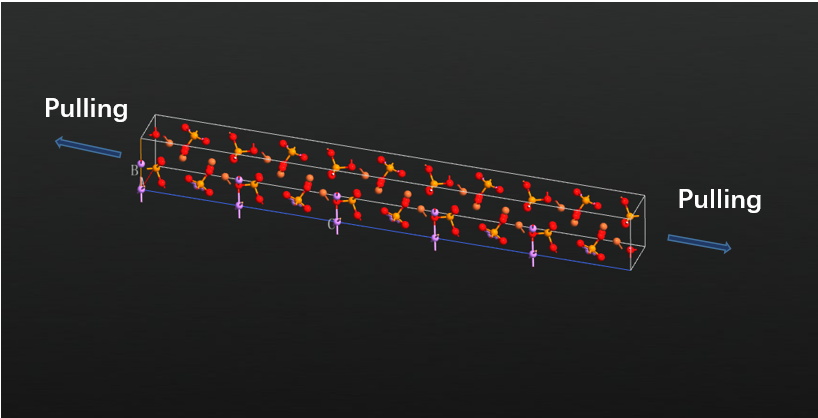
\includegraphics[width=\textwidth]{MD.png}
	\caption{$LiFePO_4$晶体的应力应变响应的分子动力学模拟} 
	\label{fig:md}
\end{figure}
\subsection{模拟过程和结果}
模拟的体系如图\ref{fig:md}所示,在两侧施加变形,进行体系弛豫,并统计出应力情况则可以得到应力-应变曲线。模拟结果见图\ref{fig:md_result}。需要注意的是,图中在起初时,随着应变增加,应力却出现了一个小的下降,这是因为起初的结构整体在z方向(图\ref{fig:md}所示的箭头方向)呈现一个压缩状态。可以看出,无论是扩散前和扩散后的结构,其在较小应变的时候($<7\%$)均有很好的线性性,即满足线弹性材料的情形,在应变到一定值($7\%$前后),出现了断裂,此处应力值有一个明显的下降。由此可以说明,由于锂离子扩散所引起的活性材料的体积变化很容易引起颗粒的断裂乃至失效。可以做一个简单的估算,对于特征尺寸为$x$的晶体,如果产生$\delta x$的形变,则其体积变化为:
\begin{equation}
\Delta V = [(x+\delta x)^3 - x^3]/x^3 = (1+ \delta x/x)^3 -1
\end{equation}
而在本文的模拟中,假设可以取$\delta x/x = 0.07$,则求得$\Delta V=0.225$,也就是说大概可以承受$22.5\%$的体积变化而不发生断裂,而实际的电池循环过程中其体积变化却有可能超出这个范围\cite{Zhang2017Chemomechanical}。

\begin{figure}
	\centering   
	\includegraphics[width=\textwidth]{initial.png}
	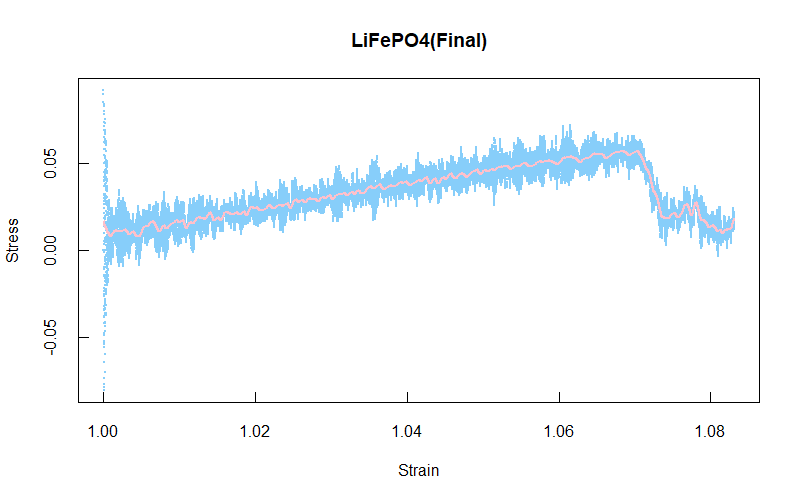
\includegraphics[width=\textwidth]{Final.png}
	\caption{$LiFePO_4$晶体的应力应变响应及断裂行为的分子动力学模拟} 
	\label{fig:md_result}
\end{figure}

\section{总结和结论}
本章首先应用第一性模拟DFT方法求解锂离子沿着$LiFePO_4$晶体的两个方向扩散的扩散路径及其对应结构,并分别求出其势垒从而比较其扩散难易得出主要的扩散方向,这也同时可以通过对于化学反应速率的比较得出一致的结论。基于得到的扩散过程的结构,首先可以求出求弹性常数,从而可以进一步求出三个方向的杨氏模量和体弹模量乃至剪切模量,从而分析晶体力学特性在扩散过程中的变化。根据模拟和比较,锂离子的扩散行为和晶体的力学特性的耦合特性,在整个扩散过程中,杨氏模量会有最高$23\%$的减小。另外,通过分子动力学模拟的方法对于锂离子扩散前后的构型进行应变加载,统计测出其应力-应变曲线,并成功观测到了材料的断裂和塑性行为。 特别地在模拟中观测到在应变小于10\%时就会发生材料的断裂,而实际上所观测到的在循环过程中电极的体积膨胀所产生的应变要显著高于此值。\\
\indent 在活性颗粒的层次,其力学行为和电化学特性密切相关。未来需要开展进一步诸如考虑电极老化等因素对于力学特性的影响;另外,进一步考虑胶层的作用将形成一个更加复杂的多界面,多层次的混合多物理场体系,对于这一体系的力学-电化学-热学特性的耦合研究需要进一步的开展。